%%%%%%%%%%%%%%%%%%%%%%%%%%%%%%%%%%%%%%%%%%%%%%%%%%%%%%%%%%%%%%%%%%%%%%%%%%%%%%%%%%%%%%%%%%%%
%%
%% Chapter 2 : Background
%%
%%      * Should give the necessary info/math/tools to understand the proposal
%%
%%  BASIC STRUCTURE :
%%
%%      a. DRL overview
%%            * RL definition
%%            * RL mathematical problem formulation
%%            * RL methods
%%              > Value based methods
%%                  - Exact methods using DP (planning by DP)
%%                  - Model free prediction (MonteCarlo and TD learning)
%%                  - Model free control (MonteCarlo, SARSA and Q-learning)
%%              > Policy based methods
%%                  - Policy gradients
%%                  - Actor Critic methods
%%            * RL with function approximation
%%            * DeepRL overview (DQN, PPO)
%%
%%      b. Simulated environments (talk about ALE, Gym)
%%          * Why is this important?
%%          * Some success stories
%%
%%      c. Simulated environments for robot locomotion
%%          * Physics engines
%%          * Robot representations
%%              - Kinematic trees
%%              - Model formats (urdf,mjcf,sdf)
%%              - Actuation models
%%          * Generic framework architecture
%%
%%%%%%%%%%%%%%%%%%%%%%%%%%%%%%%%%%%%%%%%%%%%%%%%%%%%%%%%%%%%%%%%%%%%%%%%%%%%%%%%%%%%%%%%%%%%
\chapter{Background}
\label{ch:background}

%%%%%%%%%%%%%%%%%%%%%%%%%%%%%%%
%   Figures for chapter 2
%%%%%%%%%%%%%%%%%%%%%%%%%%%%%%%

\newcommand{\figrlloop}{
    \begin{figure}
        \centering
        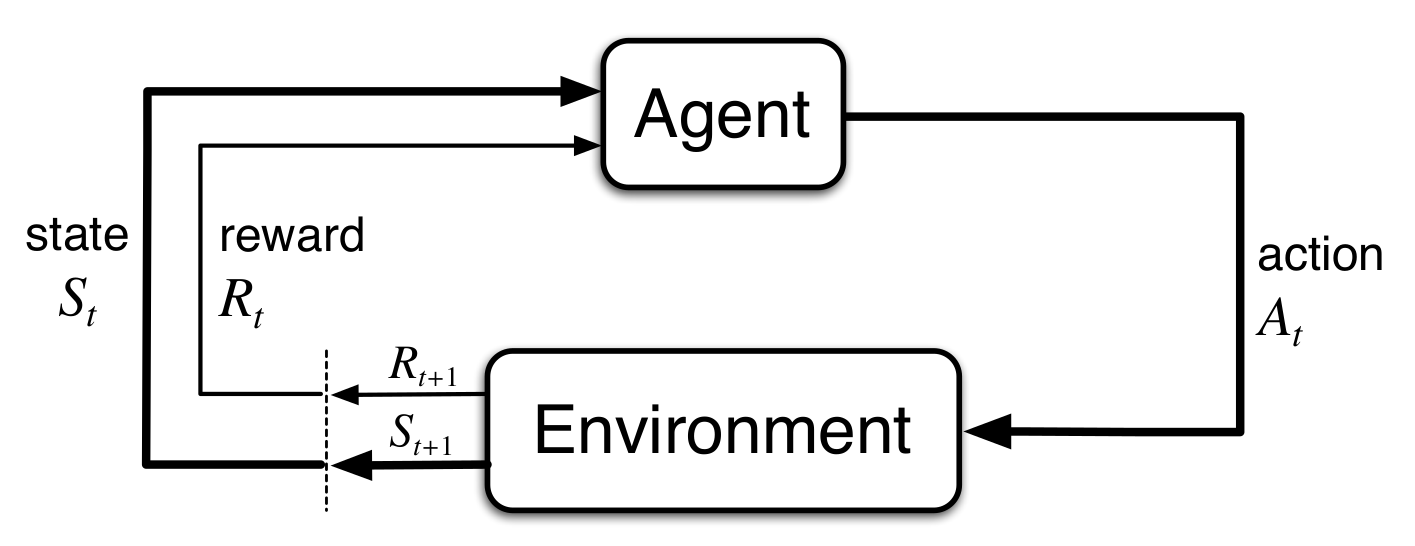
\includegraphics[width=5in]{./chapters/chapter_2/imgs/img_rl_loop.png}
        \caption{Agent-Environment interaction loop}
        \label{fig:ch2_rlloop}
    \end{figure}
}

\newcommand{\figdrlsamplesFirst}{
    \begin{figure}
        \centering
        \begin{subfigure}[b]{0.4\textwidth}
            \centering
            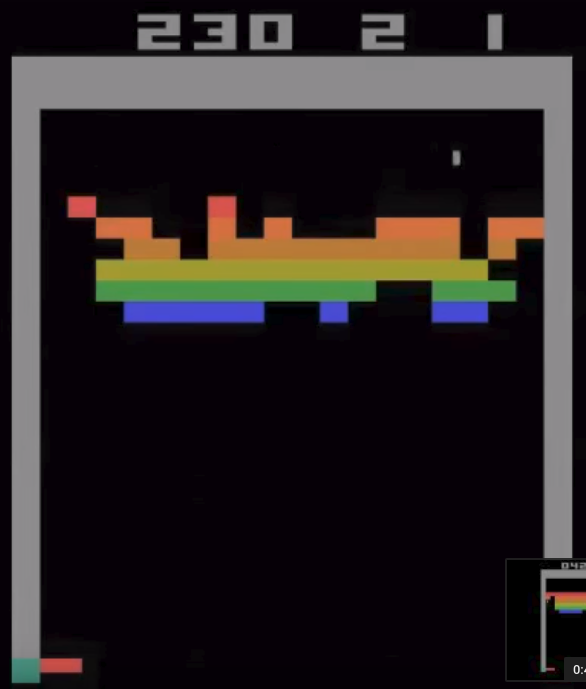
\includegraphics[width=0.9\textwidth]{./chapters/chapter_2/imgs/img_dqn_breakout.png}
            \caption{}
            \label{fig:ch2_dqn_breakout}
        \end{subfigure}
        \begin{subfigure}[b]{0.4\textwidth}
            \centering
            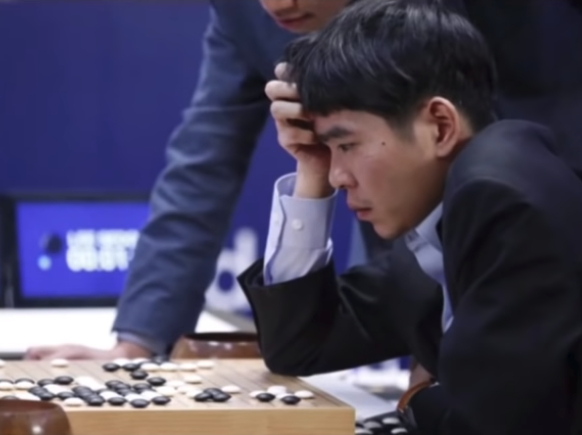
\includegraphics[width=0.9\textwidth]{./chapters/chapter_2/imgs/img_alphago.png}
            \caption{}
            \label{fig:ch2_alphago}
        \end{subfigure}
        \caption{Some DeepRL success stories: (a) DQN agent playing atari breakout [@CITE],
                                              (b) AlphaGo playing against Go champion Lee Sedol [@CITE]}
        \label{fig:ch2_drl_stories_1}
    \end{figure}
}

\newcommand{\figdrlsamplesSecond}{
    \begin{figure}
        \centering
        \begin{subfigure}[b]{0.3\textwidth}
            \centering
            
\includegraphics[width=0.9\textwidth]{./chapters/chapter_2/imgs/img_emergence_of_locomotion.png}
            \caption{}
            \label{fig:ch2_emergence_of_locomotion}
        \end{subfigure}
        \begin{subfigure}[b]{0.3\textwidth}
            \centering
            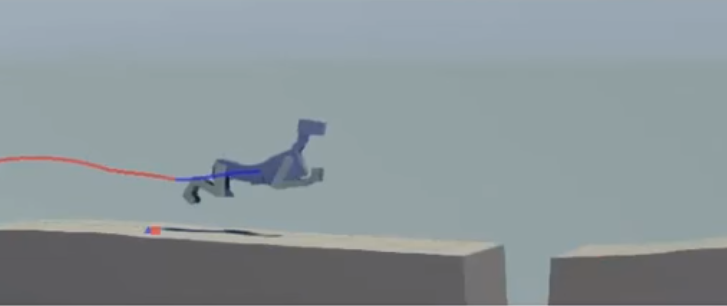
\includegraphics[width=0.9\textwidth]{./chapters/chapter_2/imgs/img_deepterrainrl.png}
            \caption{}
            \label{fig:ch2_deepterrainrl}
        \end{subfigure}
        \begin{subfigure}[b]{0.3\textwidth}
            \centering
            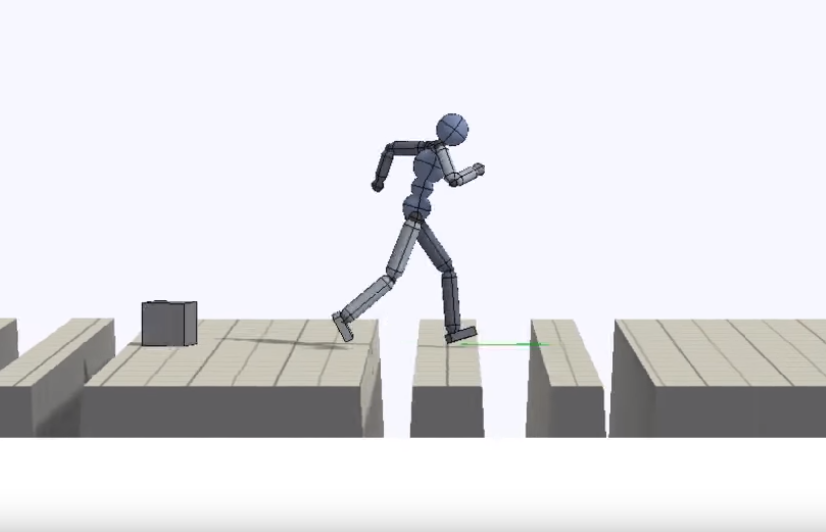
\includegraphics[width=0.9\textwidth]{./chapters/chapter_2/imgs/img_deepmimic.png}
            \caption{}
            \label{fig:ch2_deepmimic}
        \end{subfigure}
        \caption{Some DeepRL success stories: (a) Deepmind's agent running in a simulated environment [@CITE],
                                              (b) Simulated dog running in a course with obstacles [@CITE],
                                              (c) Simulated character running in an obstacle course, while 
                                                  mimicking humans' natural motion [@CITE]}
        \label{fig:ch2_drl_stories_2}
    \end{figure}
}

\newcommand{\figdrlsamplesThird}{
    \begin{figure}
        \centering
        \begin{subfigure}[b]{0.3\textwidth}
            \centering
            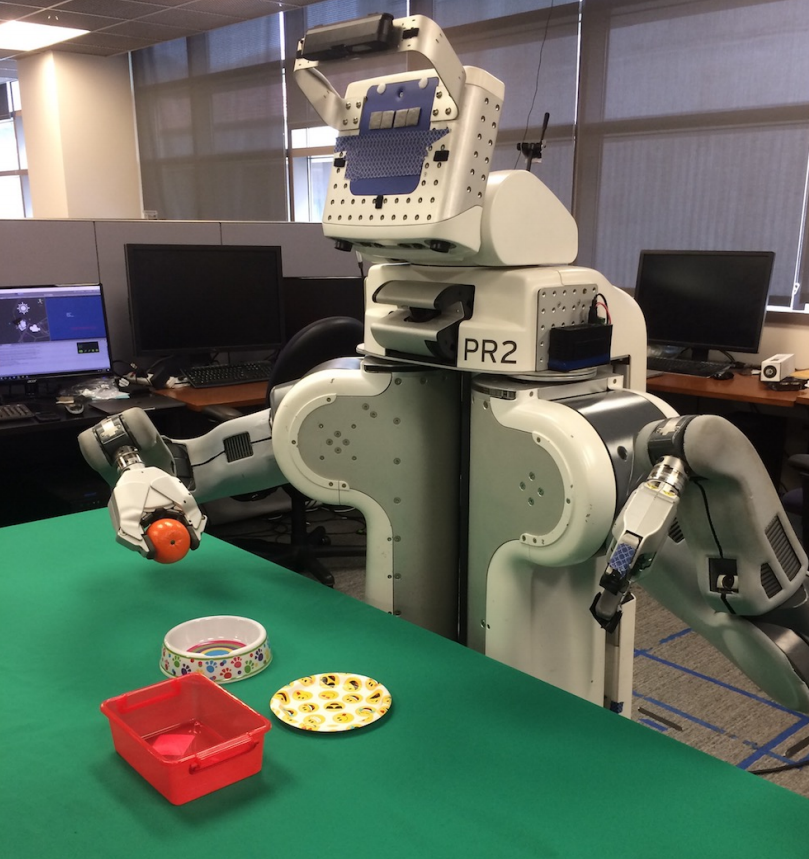
\includegraphics[width=0.9\textwidth]{./chapters/chapter_2/imgs/img_visual_motor_control.png}
            \caption{}
            \label{fig:ch2_visual_motor_control}
        \end{subfigure}
        \begin{subfigure}[b]{0.3\textwidth}
            \centering
            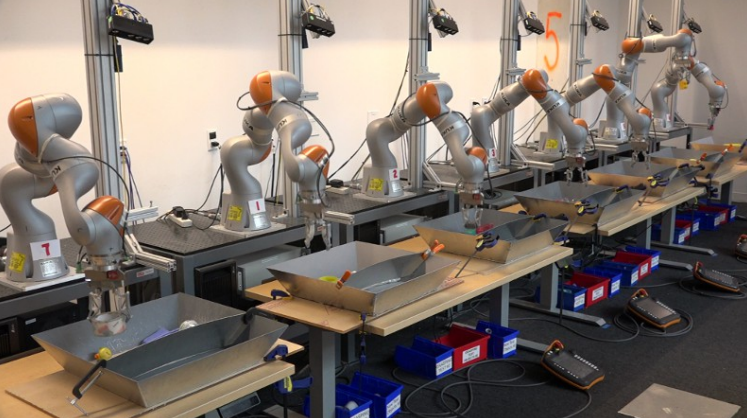
\includegraphics[width=0.9\textwidth]{./chapters/chapter_2/imgs/img_vision_based_robotics.png}
            \caption{}
            \label{fig:ch2_vision_based_robotics}
        \end{subfigure}
        \begin{subfigure}[b]{0.3\textwidth}
            \centering
            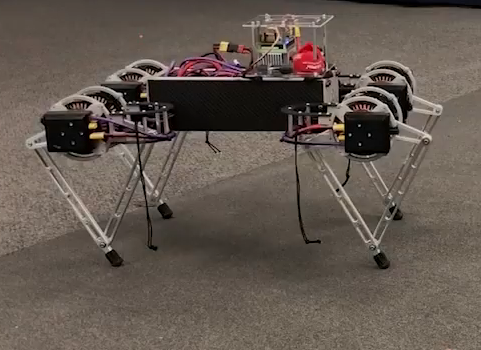
\includegraphics[width=0.9\textwidth]{./chapters/chapter_2/imgs/img_sim_2_real.png}
            \caption{}
            \label{fig:ch2_sim_2_real}
        \end{subfigure}
        \caption{Some DeepRL success stories: (a) PR2 robot learning manipulation tasks [@CITE],
                                              (b) Learning more manipulation tasks using lots of robots [@CITE],
                                              (c) Quadruped running in the real world [@CITE]}
        \label{fig:ch2_drl_stories_3}
    \end{figure}
}

\newcommand{\figMdpSamples}{
    \begin{figure}
        \centering
        \begin{subfigure}[b]{0.9\textwidth}
            \centering
            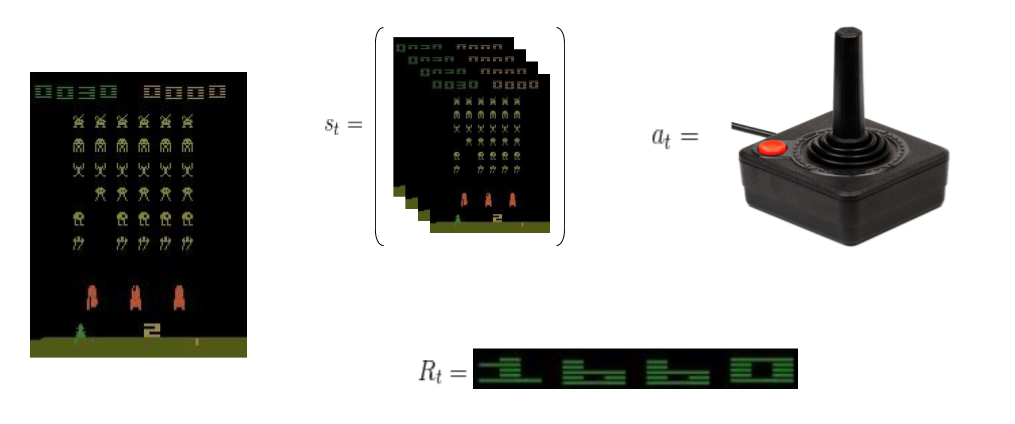
\includegraphics[width=0.9\textwidth]{./chapters/chapter_2/imgs/img_rl_mdp_atari.png}
            \caption{}
            \label{fig:ch2_mdp_sample_atari}
        \end{subfigure}

        \centering
        \begin{subfigure}[b]{0.9\textwidth}
            \centering
            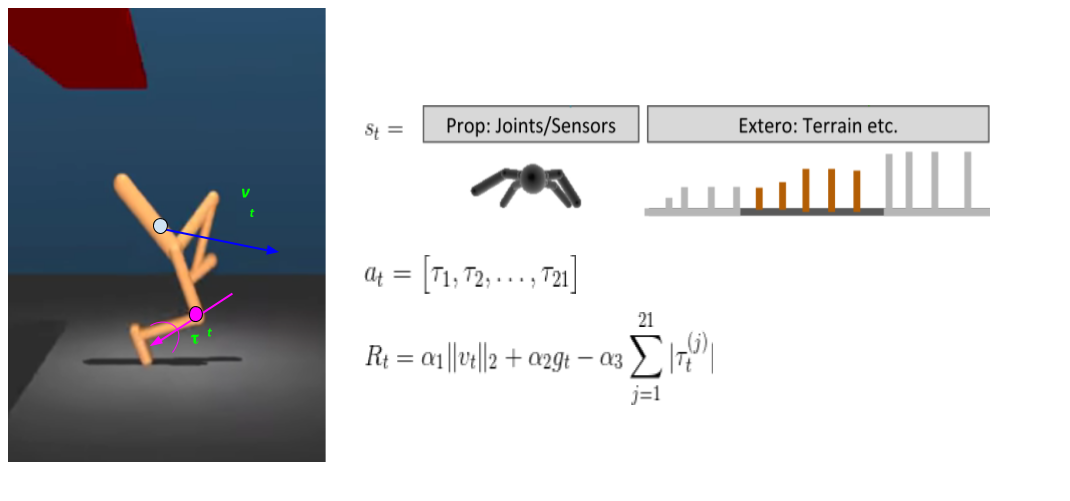
\includegraphics[width=0.9\textwidth]{./chapters/chapter_2/imgs/img_rl_mdp_locomotion.png}
            \caption{}
            \label{fig:ch2_mdp_sample_locomotion}
        \end{subfigure}
        \caption{Some examples of MDPs: (a) MDP modelling an Atari game. 
                                        (b) MDP modelling a locomotion task.}
        \label{fig:ch2_mdps_samples}
    \end{figure}
}

\newcommand{\figRlPolicies}{
    \begin{figure}
        \centering
        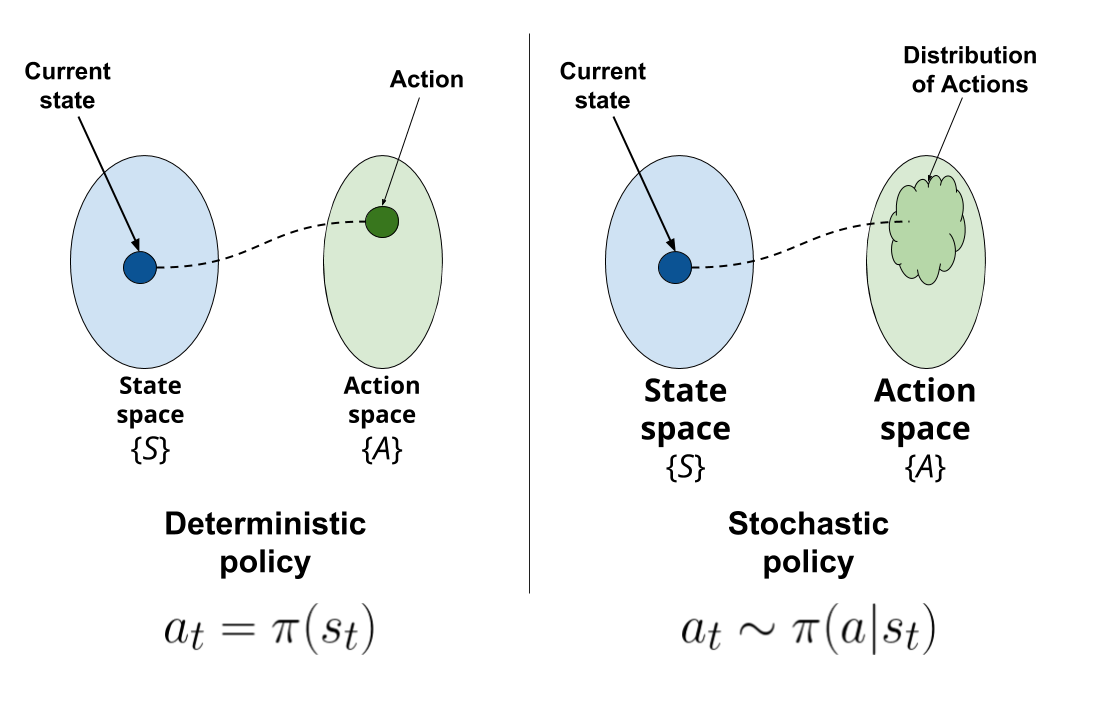
\includegraphics[width=0.9\textwidth]{./chapters/chapter_2/imgs/img_rl_policies.png}
        \caption{Differences between deterministic and stochastic policies.}
        \label{fig:ch2_rl_policies_differences}
    \end{figure}
}

\newcommand{\figRlMethodsLandspace}{
    \begin{figure}
        \centering
        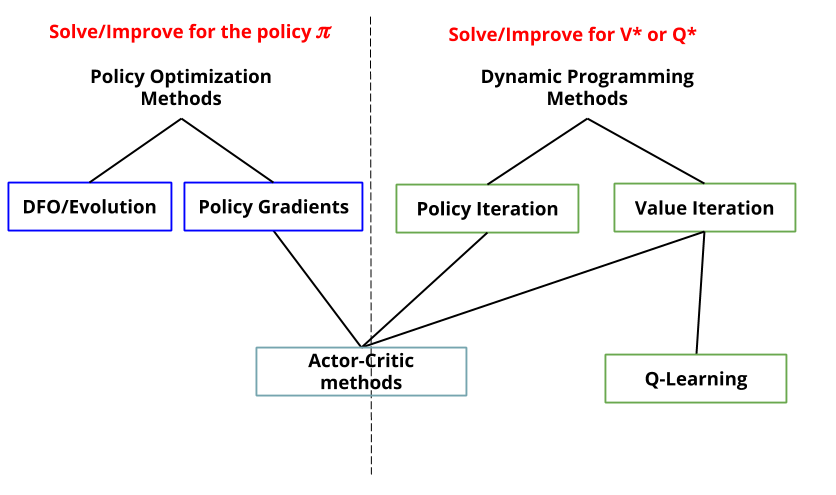
\includegraphics[width=0.9\textwidth]{./chapters/chapter_2/imgs/img_rl_methods.png}
        \caption{RL solution methods landspace. \textbf{Value-based methods} (right) solve for the policy 
                 indirectly, whereas \textbf{Policy-based methods} (left) solve for the policy directly.}
        \label{fig:ch2_rl_policies_differences}
    \end{figure}
}

\newcommand{\figRlPolicyGradientsIntuition}{
    \begin{figure}[!b]
        \centering
        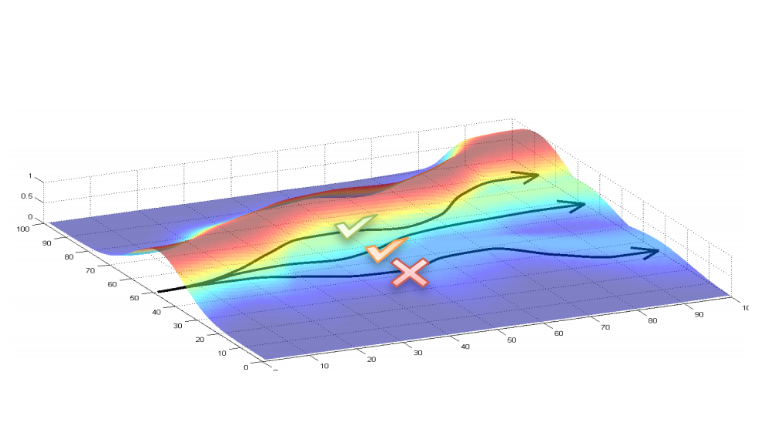
\includegraphics[width=0.8\textwidth]{./chapters/chapter_2/imgs/img_rl_pg_intuition.png}
        \caption{Intuition behind Policy Gradients. Actions that yield good trajectories are encouraged}
        \label{fig:ch2_rl_pg_intuition}
    \end{figure}
}

\newcommand{\figRlPolicyParametrization}{
    \begin{figure}
        \centering
        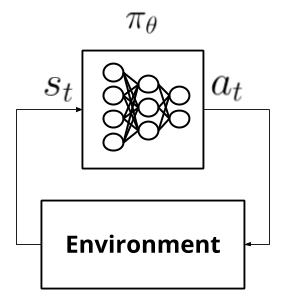
\includegraphics[width=0.3\textwidth]{./chapters/chapter_2/imgs/img_policy_parametrization.png}
        \caption{Parametrization of a policy $\pi$ using a Neural Network}
        \label{fig:ch2_rl_policy_parametrization}
    \end{figure}
}

\newcommand{\figALEgames}{
    \begin{figure}[H]
        \centering
        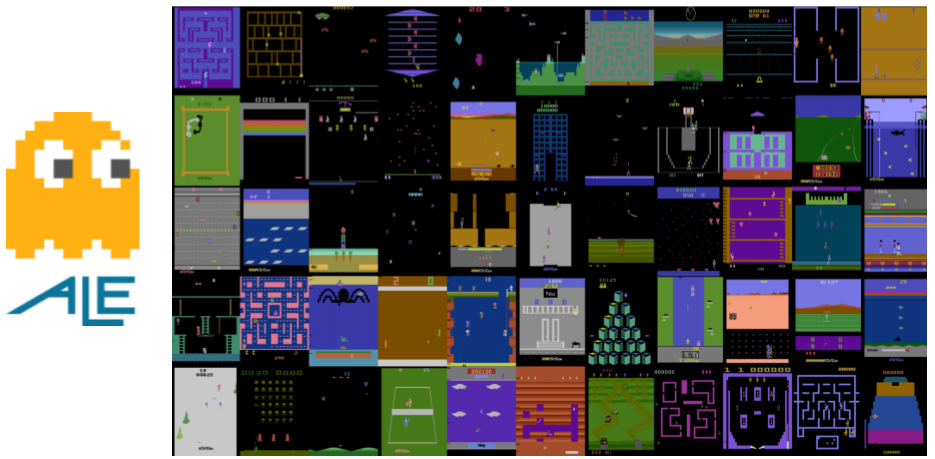
\includegraphics[width=0.6\textwidth]{./chapters/chapter_2/imgs/img_atari_learning_environment.png}
        \caption{Games in the Atari Learning Environment.}
        \label{fig:ch2_ale_games}
    \end{figure}
}

\newcommand{\figOpenAIEnvs}{
    \begin{figure}[H]
        \centering
        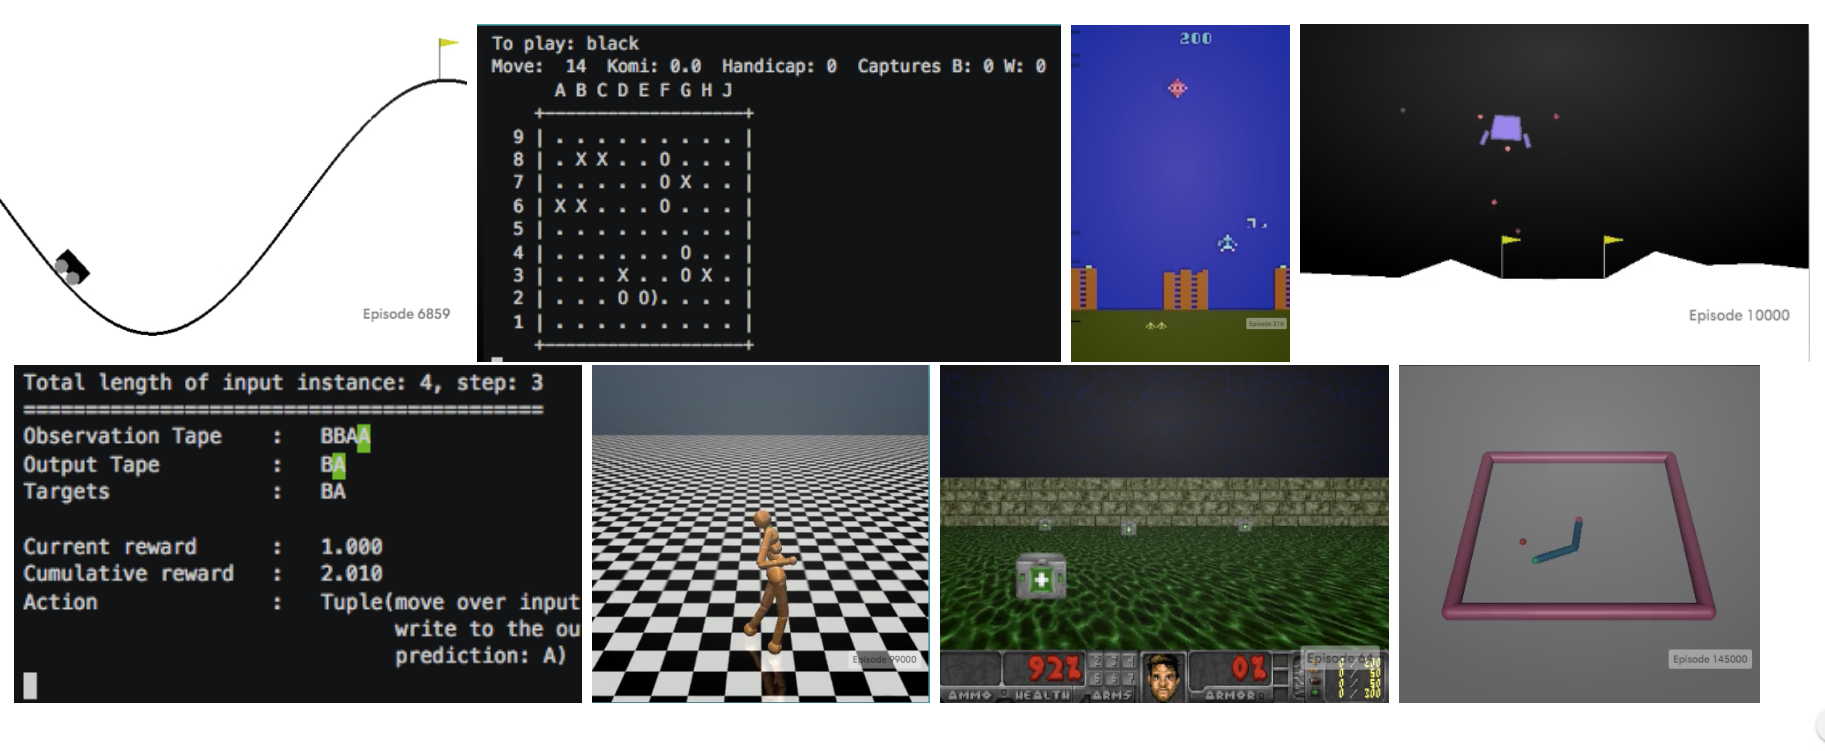
\includegraphics[width=0.9\textwidth]{./chapters/chapter_2/imgs/img_openai_gym_envs.png}
        \caption{Environments in OpenAI Gym.}
        \label{fig:ch2_gym_envs}
    \end{figure}
}

\newcommand{\figDeepmindLabEnvs}{
    \begin{figure}[H]
        \centering
        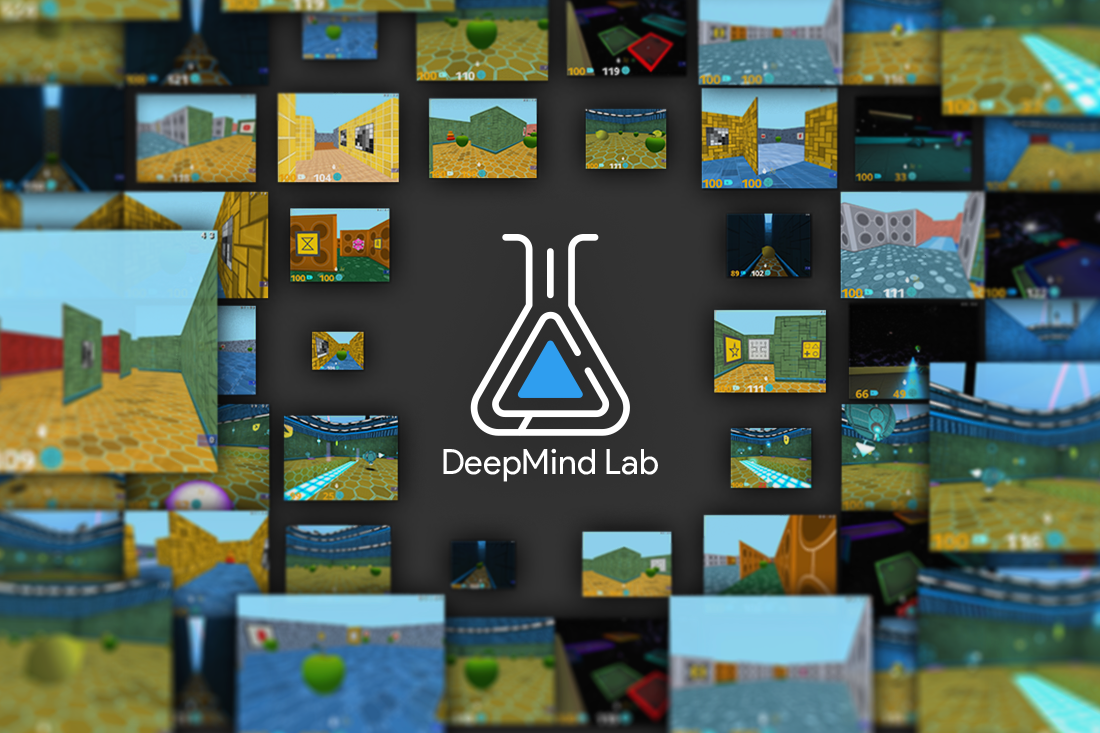
\includegraphics[width=0.7\textwidth]{./chapters/chapter_2/imgs/img_deepmind_lab.png}
        \caption{Environments in Deepmind Lab}
        \label{fig:ch2_deepmind_lab}
    \end{figure}
}

In this chapter we we will give an overview of the core concepts needed to
understand the following chapters in this document. These include:


\begin{itemize}
    \item A brief overview of the field of \textbf{Deep Reinforcement Learning}, where
          we describe some concepts of Reinforcement Learning, Deep Learning, and Deep
          Reinforcement Learning.
    \item An overview of \textbf{learning environments}, which are a key component of
          the Reinforcement Learning framework. We analyze why are they important 
          and some examples used in current Deep Reinforcement Learning research.
    \item A more specific overview of \textbf{learning environments for robot locomotion}, 
          what are their components, and some concepts about their design. This is
          intended for the first half of the proposal which consists of making this type
          of learning environments.
\end{itemize}


\section{Deep Reinforcement Learning}

At a very high level Deep Reinforcement Learning (DeepRL) could be thought as a combination 
of current Deep Learning (DL) models and techniques, with the framework of Reinforcement 
Learning (RL), to solve complex RL problems. This combination has given impressive 
results over the past few years, like being able to play a suite of atari games [@CITE], 
beating the world Go champion [@CITE], making simulated characters develop locomotion
skills [@CITE,@CITE,@CITE], and being able to learn manipulation and locomotion tasks in 
real-world robotics platforms [@CITE,@CITE], just to name a few.

\figdrlsamplesFirst

\figdrlsamplesSecond

\figdrlsamplesThird

Let's start by defining Reinforcement Learning and classic solutions methods, and then
see how Deep Learning fits into this framework by providing a way to capture representation
in the context of function approximation.

\subsection{Reinforcement Learning}

Reinforcement Learning is an overloaded term that encloses both a \textbf{learning approach}
and the \textbf{algorithms} that solve problems in this paradigm. RL as a learning approach
is a learning paradigm, like supervised and unsupervised learning, with the difference that
instead of learning from a curated dataset (like in supervised learning) or learning an underlying
structure of unlabeled incoming data (like in unsupervised learning), in RL we learn by interactions
with an environment.

In Figure @FIG-2.4 we show the Agent-Environment interaction loop. This represents
the way an agent in a certain \textbf{state} $S_{t}$ (a certain modeled configuration) interacts 
with its environments by means of some \textbf{action} $A_{t}$, and models how the environment 
responds by giving the agent a \textbf{reward} $R_{t+1}$ (basically a score for its interaction) 
and a \textbf{new state} $S_{t+1}$ (obtained from the environment dynamics).

\figrlloop

We can formalize this setting with Markov Decision Processes (MDPs), which is a framework
that we can use to model sequential decision making problems with uncertainties.

\begin{definition}
    A Markov Decision Process (MDP) is a 5-tuple of the following components:
    \begin{itemize}
        \item A set of states $s \in S$
        \item A set of actions $a \in A$
        \item A transition model $T(s',s,a) = P(s'|s,a)$
        \item A reward function $R(s',s,a)$
        \item A discount factor $\gamma$
    \end{itemize}
\end{definition}

We have already talked about some of the components of an MDP (state, action, reward).
The remaining components consist of: a transition model of the environment, $P(s'|s,a)$
which basically models the environment's dynamics into a single conditional probability
distribution, and a discount factor $\gamma$ that models that rewards in the future might have
less importance than rewards now (discounting like when dealing with money). Some examples 
of problems in RL formulated in the MDP framework are shown in Figure @FIG-2.5.

\figMdpSamples

The objective of the agent is to maximize the expected sum of rewards it gets from
its interaction with the environment. To achieve this it has to come up with a
way to select the appropiate actions in a given situation, which in this case is given
by the state of the agent. To formalize this, let's define some extra concepts:

\begin{itemize}
    \item \textbf{Returns}, which is a more compact notation to express the sum of rewards.
    \item \textbf{Policies}, which are the way an agent picks its actions, meaning they
          are the solution to our RL problem.
\end{itemize}

\newpage

\begin{definition}
    The return $G_{t}$ is defined as the sum of rewards an agent gets from its
    interactions starting at timestep $t$.
    \begin{equation}
        G_{t} = \sum_{k=0}^{\infty} \gamma^{k} R_{t+k+1}
    \end{equation}
\end{definition}

\begin{definition}
    A deterministic policy $\pi(s)$ is defined as a mapping between states $s \in S$
    to action $a \in A$.
    \begin{equation}
        \pi : S \rightarrow A
    \end{equation}
\end{definition}

\begin{definition}
    An stochastic policy $\pi(a|s)$ is defined as a conditional probability distribution over
    states $s \in S$ of a certain action $a \in A$.
    \begin{equation}
        \pi : S \times A \rightarrow [0,1]
    \end{equation}
\end{definition}

\figRlPolicies

Figure @FIG-2.6 shows the differences between an stochastic policy and a deterministic
policy. We can reformulate the objective of the agent into the following: \textit{An agent's objective
in the RL setup is to maximize the expected return $\mathbb{E} \lbrace G_{t} \rbrace$ it
can get from its interactions with the environment by finding the best policy $\pi$, which
we call optimal policy, and denote by $\pi^{*}$}

\begin{equation}
    \pi^{*} = \arg \max_{\pi} \mathbb{E}_{\pi} \lbrace G_{t} \rbrace
\end{equation}

\subsection{Solution methods}

\figRlMethodsLandspace

To solve an MDP there are various methods that can be used. Most of them are
summarized in the categories shown in Figure @FIG-2.7. These include:

\begin{itemize}
    \item \textbf{Value based methods}, which try to solve for some auxiliary
          functions, called \textit{State-value} and \textit{Action-value} functions
          and then extract the solution directly.
    \item \textbf{Policy based methods}, which solve for the policy directly. These methods
          make use of some parametrization of the policy via some function approximator
          (like a Neural Network), and then search for the parameters of this policy
          by optimizing for the expected return.
\end{itemize}

Most of the current methods used are Policy based methods, specially in the context
of robot locomotion. In the following section we will cover some concepts used when
using policy based methods.

\subsection{Policy Optimization}

As described earlier, policy based methods try to solve for the parameters $\theta$
of a parametrized policy $\pi_{\theta}$ such that this policy maximizes the expected
return the agent gets from its interactions with the environment.

\begin{equation}
    \theta = \arg \max_\theta \mathbb{E}_{\pi_{\theta}} \lbrace G_{t} \rbrace
\end{equation}

One way to solve this optimization problem is to apply Derivative Free Optimization
methods, like evolutionary algorithms. These black box optimization methods would
search for the right set of parameters that satisfy the objective we are requesting.

We will focus in Gradient based optimization methods, which make use of gradient
ascent to search for the right set of parameters. The kind of gradient used in this
case is an estimate of the gradient of this expectation objective, which we can sample
using sample trajectories of interaction, and then use it with an optimizer like
SGD. Let's introduce some extra concepts and then present this gradient estimate,
and the base form of the Policy Gradients algorithms.

\begin{definition}
    A trajectory $\tau$ is defined as a consecutive sequence of states, actions 
    and rewards experienced by an agent over its interactions with the environment.
    \begin{equation}
        \tau = \lbrace s_{0},a_{0},r_{1},s_{1},a_{1},r_{2},\hdots,s_{H-1},a_{H-1},r_{H} \rbrace
    \end{equation}
\end{definition}

\begin{definition}
    We define the return over a trajectory $G(\tau)$ as the discounted sum of
    rewards obtained in that trajectory.
    \begin{equation}
        G(\tau) = \sum_{t=0}^{H} \gamma^{t} r_{t+1}
    \end{equation}
\end{definition}

We then can reformulate the objective we want to optimize for using this new notation.
Recall that the agent tries to its maximize expected return, so we can define this as
an objective $J$ that depends on the parameters of our policy as follows:

\begin{equation}
    J(\theta) = \mathbb{E}_{\tau \sim p(\tau;\theta)}[G(\tau)]
\end{equation}

Where $p(\tau;\theta)$ is a probability distribution of trajectories, induced by
the parameters of our policy $\theta$ (recall that the agent sees what its policy allows)